\documentclass{sig-alternate}

\usepackage{amsmath,mathtools,nccmath}
\usepackage{paralist}
\usepackage{tikz}
\usetikzlibrary{matrix,arrows,shapes,calc}

\newtheorem{definition}{Definition}
\newtheorem{example}{Example}
\newtheorem{theorem}{Theorem}
\newtheorem{lemma}{Lemma}

\newcommand{\ifthenelse}[3]{\mathbf{if}\ #1\ \mathbf{then}\ #2\ \mathbf{else}\ #3\ \mathbf{fi}}
\newcommand{\pvec}[1]{\vec{#1}\mkern2mu\vphantom{#1}} %for primed vector (by egreg)


\begin{document}


\title{Bounded Model Checking of Distributed Cyber-Physical Systems 
using SMT over Reals
(tentative)
%\titlenote{For use with ACM\_PROC\_ARTICLE-SP.CLS. Supported by ACM.}
}

\numberofauthors{4}
\author{
Kyungmin Bae, Sicun Gao, Soonho Kong, Edmund M. Clarke\\
\affaddr{Department of Computer Science}\\
\affaddr{Carnegie Mellon University}
}

\maketitle
\begin{abstract}
Many cyber physical systems %such as airplanes and cars, 
are \emph{distributed hybrid systems}
where distributed controllers communicate with each other via a network
and govern physical entities with continuous dynamics.
For model checking \emph{virtually synchronous} cyber physical systems,
the PALS methodology \cite{pals-rtss09,mr-pals-journal,pals-tcs} 
has been proposed to 
reduce the combinatorial complexity  caused by the system's concurrency.
But its application to distributed hybrid systems is quite limited 
due to  
real-number inputs and parameters, 
imprecisions of the local clocks, 
correlation between physical entities,
nonlinear differential equations, etc.
%
This paper explains how a wide range of distributed hybrid systems,
involving non-linear differential equations and real number inputs and parameters,
can be effectively verified using a $\delta$-complete SMT solver over reals,
together with Multirate PALS.
We illustrate our method with two nontrivial distributed hybrid system case studies.
\end{abstract}




%
\section{Introduction}

\emph{Virtually synchronous} cyber physical systems (CPS) are given by  a number of 
\emph{periodic} controllers that communicate  asynchronously with each other through a network,
but that obey hard real-time synchronization constraints for their correctness.
A controller in the system may interact with its  local \emph{physical environment}
whose continuous dynamics is modeled by differential equations
(e.g., avionics, aerospace, 
automotive, robotics, etc). 
%
In practice, the design of such systems is very hard because of race 
conditions, clock skews, network delays, and execution times,  in addition to the 
usual difficulties for non-distributed CPS.
Furthermore, the model checking 
of a virtually synchronous CPS becomes typically unfeasible 
due to the combinatorial explosion caused by 
the system's concurrency.
% Although DCPS very widely appears in many practical applications, 
%such as avionics, aerospace, automotive, robotics, etc, 
%formal verification of DCPS is very restrictive even these days.
The PALS (physically asynchronous, but logically synchronous) methodology 
\cite{pals-rtss09,mr-pals-journal,pals-tcs} has been
developed to reduce the system complexity of a virtually 
synchronous CPS,
provided that the network infrastructure defines \emph{performance bounds} %$\Gamma$ 
on  computation times, network delays, and imprecisions of the local clocks.


However, 
the model checking verification of distributed hybrid systems with continuous dynamics
is still limited even with PALS by the following reasons.
First, inputs or parameters of CPS can be any real numbers in a certain bound.
That is, model checking using concrete inputs and parameters 
cannot verify the safety of the system in this case,
although quite useful for finding erroneous behaviors.
Second, the continuous behavior of the system depends on
the local clocks of the distributed components, 
because they can read their sensor values according to the local clocks;
but the underlying infrastructure can only guarantee that the imprecisions 
between the local clocks are up to a certain bound $\epsilon > 0$.
Similarly, model checking using specific local clocks cannot verify 
the correctness of the system.
Third, the continuous behavior of a CPS often 
involves \emph{nonlinear} ordinary differential equations
which do not provide exact solutions in general.
A typical approach of using numerical simulations
cannot of course verify the correctness.


Moreover, in distributed hybrid systems, 
a local physical environment of one component
may \emph{immediately} affect the behavior of 
a local environment of another component,
when they are \emph{physically correlated} to each other.
For example, if we consider two adjacent rooms with thermostat controllers, 
the temperature of one room may immediately affect 
the temperature of the other room, unless they are perfectly insulated.
Such a behavior cannot be properly captured 
by a network communication between distributed components
in the previous PALS framework,
because components are assumed to be periodically executed in PALS.
Therefore, it is nontrivial to specify the behavior of a local environment
of a single component  \emph{in a modular way} 
without taking account into the entire system.
Also, how can we verify the safety of distributed hybrid systems in these cases?

This paper shows that all the above-mentioned problems
in verifying distributed hybrid systems can be dealt with by:
\begin{inparaenum}[(i)]
	\item modeling the behavior of physical environments as 
	 logical constraints (over reals), and
	\item performing bounded model checking with \emph{delta-complete SMT} solving
	to verify the safety of the system.
\end{inparaenum}
%
An SMT (satisfiability modulo theories) problem is to check
the satisfiability of first-order formulas with respect to 
certain (decidable) logical  theories.
The \texttt{dReal} \cite{DBLP:conf/cade/GaoKC13} is an SMT solver 
to automatically check the satisfiability of first-order formulas over reals 
with non-linear   ordinary differential equations,
up to any given precision $\delta > 0$
(which is shown to be decidable in
\cite{DBLP:conf/cade/GaoAC12,DBLP:conf/fmcad/GaoKC13}).
The basic idea is to reduce the verification problem of a CPS
with physical environment constraints
to the SMT problem for reals and (non-linear)  differential equations.





More precisely,
our main contribution in this paper can be summarized as follows:

\begin{itemize}
	\item We show that the behavior of physical environments
	in distributed CPS
	can be precisely modeled in a modular way
	by logic constraints of physical parameters,
	even when they are physically correlated to each other.
	
	
	\item We show that the verification problem of distributed CPS 
	can be reduced to 
	checking the satisfiability of logic formulas over real numbers.
	%based on the bounded model checking framework.
	We also show how we can deal with 
	arbitrary real number inputs and parameters, 
	and imprecisions of the local clocks.
	
	
	\item We explain how the satisfaction of the generated logic formula 
	can be decided using \texttt{dReal}
	(the formula itself may be beyond the class of formulas directly handled
	in the current input language of \texttt{dReal}).
	

	\item We illustrate two case studies, namely, a distributed controller for turning
	an airplane, and a distributed robot controller for simulating a Turing machine.
\end{itemize}

The rest of our paper is organized as follows.
%
Section~\ref{sec:dcps-design}
briefly recalls the PALS methodology,
and shows how a wide range of distributed CPS
can be specified in this framework, by expressing 
the continuous behavior as logical constraints over real numbers.
Section~\ref{sec:dcps-bmc}
presents the bounded model checking of a CPS using SMT over reals,
and
%Section~\ref{sec:component-dReal} 
then explains how such SMT problems,
which may involve uninterpreted functions for reals,
can be dealt with by \texttt{dReal}.
Section~\ref{sec:case-studies} presents two case studies 
and their verification using our methods.
Finally,
Section~\ref{sec:related-work} explains some related work,
and 
Section~\ref{sec:concl} presents some concluding remarks.

\section{Distributed CPS Design}
\label{sec:dcps-design}

We consider \emph{virtually synchronous} cyber physical systems (CPS)
that are implemented as networked devices
and are 
controlled by a hierarchy of multirate distributed controllers. 
%
The devices and controllers may operate at different rates,
where the period of a higher-level component is 
a multiple of the period of its connected (fast) component.
The design and verification of such virtually synchronous CPS is 
very hard due to asynchronous communication, network delays,
clock skews, plus the state space explosion caused by the system's concurrency.
The PALS (physically asynchronous, but logically synchronous) 
methodology \cite{pals-rtss09,mr-pals-journal,pals-tcs}
can reduce the design and verification of a virtually synchronous CPS to
those of its (much simpler) synchronous version.

Consider a synchronous design $\mathcal{E}$---given by a 
collection of state machines with local clocks and different rates---and 
performance bounds
$\Gamma = (\epsilon, \alpha_{\min}, \alpha_{\max}, \mu_{\min}, \mu_{\max})$
of the underlying network infrastructure, where:
\begin{inparaenum}[(i)]
	\item the difference between a local clock of 
	each component and the global time is less than $\epsilon$;
	\item the duration for each component to process input, 
	execute a transition, and generate output is within 
	the interval $[\alpha_{\min},\alpha_{\max}]$;
	and
	\item  the point-to-point message transmission time between 
	any two components is within the interval $[\mu_{\min}, \mu_{\max}]$.
\end{inparaenum}
The PALS transformation then generates
the corresponding distributed asynchronous design 
$\mathcal{A}(\mathcal{E}, T, \Gamma)$,
with $T$ a global period,
in which
  $\mathcal{E}$ and $\mathcal{A}(\mathcal{E}, T, \Gamma)$
satisfy 
the same temporal logic 
properties \cite{mr-pals-journal,pals-tcs}.
Therefore, we can simply design and verify a synchronous model $\mathcal{E}$,
and then PALS can give  the \emph{correct-by-construction} distributed 
implementation $\mathcal{A}(\mathcal{E}, T, \Gamma)$ automatically.

This section first recalls a synchronous model $\mathcal{E}$
which defines a discrete behavior of CPS,
specified as a multirate synchronous composition of state machines (Section~\ref{sec:ensemble}).
To deal with the  continuous behavior of physical environments,
we specify  physical environments 
using periodic
dynamic systems together with logical constraints %of physical parameters
%logical constraints over real numbers and (nonlinear) ordinary differential equations
(Section~\ref{sec:env-const}). 
This is different from the previous approach in \cite{ftscs-journal}
where local physical environments are modeled as
usual state machines.
Any network communication between different 
distributed components
\emph{cannot be immediate} due to network delays,
and therefore
``physically correlated'' local environments---where one local environment may immediately 
affect  another environment---were not properly dealt with in the previous approach,
whereas they can  be naturally expressed by our new approach
using logical constraints.




\subsection{Discrete Synchronous Models}
\label{sec:ensemble}

The synchronous model is formally specified as
 a multirate synchronous composition of 
a collection of nondeterministic \emph{typed state machines}
 and a \emph{wiring diagram} connecting  the input and output \emph{ports} of the machines \cite{pals-tcs}.   
%
A \emph{typed machine} %$M$ with $n$ input ports and $m$ output ports
is a tuple $M = (D_i,S,D_o,\delta_M)$, with
$S$ a finite set of states,
$\delta_M \subseteq (D_i \times S) \times (S \times D_o)$ a %total 
	transition relation, and:

\begin{itemize}
	\item $D_i = D_{i_1} \times \cdots \times D_{i_n}$ an input set 
(a value to \emph{input port} $1 \leq k \leq n$ is an element of $D_{i_k}$), 
	\item $D_o =D_{o_1} \times \cdots \times D_{o_m}$ an output set
(a value from \emph{output port} $1 \leq j \leq m$ is an element of $D_{o_j}$), and
\end{itemize}

As shown in Figure~\ref{fig:ensemble},
typed machines can be composed using a wiring diagram
into a \emph{multirate machine ensemble}
$\mathcal{E} = (J_S \cup J_F, e, \{M_j\}_{j\in J_s \cup J_F}, E, \mathit{src}, \mathit{rate}, \mathit{adap})$,
 where:
 
\begin{itemize}
	\item $J_S$ and $J_F$ are sets of ``slow'' and ``fast'' machine indices,
	respectively, % ($J_S \cap J_F = \emptyset$), 
	and  $e\not\in J_S \cup J_F$ is the ``interface'' index;
		
 	\item $\{M_j\}_{j\in J_S \cup J_F}$ is  a family of typed machines;
	
	\item $E=(\mathcal{D}^e_i, \mathcal{D}^e_o)$ is the ensemble's \emph{interface}
	with $\mathcal{D}^{e}_i$   the \emph{input set} and $\mathcal{D}^{e}_o$  the \emph{output set};
	
	\item $\mathit{src}$ is  a \emph{wiring diagram} assigning to each input port $(j, n)$ 
	(port $n$ of machine $j$)  its ``source'' output port;
	
	\item $\mathit{rate}$ assigns to each fast machine 
	its \emph{rate} denoting 
	how many times faster than the slow machines; 
	and

	\item $\mathit{adap}$ assigns an \emph{input adaptor} (explained below) to each typed machine in $\{M_j\}_{j\in J_S \cup J_F}$.
\end{itemize}
%\end{definition}

\noindent
The physical environments of components are 
assumed to be already integrated with their controllers (see Section~\ref{sec:env-const}).


\begin{figure}
\centering
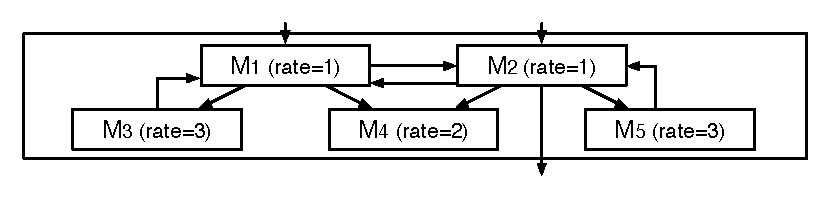
\includegraphics[clip=true,trim=0.3cm 0.4cm 0.3cm 0.4cm,width=1.0\columnwidth]{ensemble.pdf}    
\caption{A multirate ensemble.
$M_1$ and $M_2$ are slow machines, and 
%$M_3$, $M_4$, and $M_5$ are fast machines.
$\mathit{env}_4$ and $\mathit{env}_5$ are local physical environments 
of $M_4$ and $M_5$, respectively.
}  \label{fig:ensemble}
\end{figure}



The transitions of all components in an ensemble $\mathcal{E}$
are performed at the same time in lockstep for each iteration.
Each fast component $j \in J_F$ is \emph{slowed down} 
by performing $k = \mathit{rate}(j)$ internal transitions  in one synchronous step.
If a machine has a ``feedback'' wire connected to itself or to another component,
then the output becomes an input of the destination component in the \emph{next} iteration.
That is,
the \emph{synchronous composition}  of an ensemble $\mathcal{E}$
is equivalent to a single machine $M_\mathcal{E}$
whose state consists of the states of its subcomponents
and the feedback outputs \cite{mr-pals-journal,pals-tcs}.
For example, 
the synchronous composition $M_\mathcal{E}$ 
of the ensemble $\mathcal{E}$ in Figure~\ref{fig:ensemble} 
is the machine given by the outer box. 
Notice that $M_\mathcal{E}$ can appear as a component 
in another multirate ensemble, resulting in hierarchical multirate systems.

Since a fast machine performs $k$ internal transitions 
one synchronous step,
a $k$-tuple of outputs from the fast machine
must be transformed to a single input (e.g., the last value, or the average of the $k$ values)
to be read by a slow component.
Similarly,
a single output from a slow component must be transformed 
to a $k$-tuple of inputs for a fast component
(e.g., 
a $k$-tuple $(d, \bot, \ldots, \bot)$ for some ``don't care'' value $\bot$).
An \emph{input adaptor} 
$\alpha=\{\alpha_j: D'_j \rightarrow D_{i_j}\}_{j\in\{1,\ldots, n\}}$
for a typed machine $M = (D_i, S, D_o, \delta_M)$
is a family of functions which determine a desired  value 
$\alpha_j(d_j) \in D_{i_j}$ for each input 
port $j$  from an output $d_j \in D_{j}'$
of another typed machine.


%The $k$-step \emph{deceleration} of  
%a machine $M = (D_i, S, D_o, \delta_M)$ for $k \in \mathbb{N}_{>0}$
%%with $D_i =  D_{i_1}\times \cdots \times D_{i_n}$ and 
%%$D_o = D_{o_1}\times \cdots \times D_{o_m}$, 
%is defined by
%%
%$M^{ \times k} = ((D_{i_1})^k \times \cdots \times (D_{i_n})^k,\,  S,\,
%(D_{o_1})^k\times \cdots \times (D_{o_m})^k,\, \delta_{M^{ \times k}})$,
%%
%where
%\[
%\begin{multlined}
%\big((((d_{i_{1_1}}, \ldots, d_{i_{1_k}}), \ldots,(d_{i_{n_1}}, \ldots, d_{i_{n_k}})),  s), \\
%(s',((d_{o_{1_1}}, \ldots, d_{o_{1_k}}), \ldots,(d_{o_{m_1}}, \ldots,d_{o_{m_k}})) ) \big) \in \delta_{M^{ \times k}}
%\end{multlined}
%\]
%iff there exist states $s_1, \ldots, s_{k-1} \in S$ such that 
%	\begin{alignat*}{2}
%		(((d_{i_{1_1}}, \ldots, d_{i_{n_1}}), s) &,\; (s_1, (d_{o_{1_1}}, \ldots, d_{o_{m_1}}))) &&\in \delta_M \\
%		(((d_{i_{1_2}}, \ldots, d_{i_{n_2}}), s_1) &,\; (s_2, (d_{o_{1_2}}, \ldots, d_{o_{m_2}}))) &&\in \delta_M\\
%		&\vdots  &&\;\,\vdots\\
%%		(((d_{i_{1_{k-1}}}, \ldots, d_{i_{n_{k-1}}}) , s_{k-2}) &,\; (s_{k-1},(d_{o_{1_{k-1}}}, \ldots, d_{o_{m_{k-1}}}) )) &&\in \delta_M\\
%		(((d_{i_{1_{k}}}, \ldots, d_{i_{n_{k}}}), s_{k-1}) &,\; (s', (d_{o_{1_{k}}}, \ldots, d_{o_{m_{k}}}))) &&\in \delta_M.
%	\end{alignat*}

% Given an input adaptor
% $\alpha=\{\alpha_k: D'_k \rightarrow D_{i_k}\}_{k\in\{1,\ldots, n\}}$
% of a machine $M = (D_i, S, D_o, \delta_M)$,
%the \emph{adaptor closure}  is 
%a machine $M_\alpha = ((D'_1\times\cdots\times D'_n), S, D_o, \delta_{M_\alpha})$
%such that
%$((\vec{d_i}, s), (s', \vec{d_o})) \in \delta_{M_\alpha}$
%iff
%$((\alpha(\vec{d_i}), s), (s', \vec{d_o})) \in \delta_{M}$,
%where $\alpha(\vec{d}) = (\alpha_1(d_1), \ldots, \alpha_n(d_n))$.



\subsection{Continuous Physical Constraints}
\label{sec:env-const}

A state of a physical environment $E_M$ %for a machine $M$
is %in general 
represented as a tuple $\vec{v} = (v_1,v_2,\ldots,v_l) \in \mathbb{R}^l$ 
of its physical parameters $\vec{x} = (x_1,x_2, \ldots,x_l)$.
%As usual in physical dynamics,
The behavior of $E_M$
can be modeled as differential equations %for the parameters,
that specify \emph{trajectories} 
$\tau_1, \tau_2, \ldots, \tau_l$ of the parameters $\vec{x}$. %$x_1,x_2, \ldots,x_l$.
A \emph{trajectory} \cite{lynch2003hybrid} of duration $T \in \mathbb{R}_{\geq 0}$ is a function $\tau : [0,T] \rightarrow \mathbb{R}$
that defines the 
continuous behavior of a physical parameter.
% during $T \in \mathbb{R}_{\geq 0}$.
%
Let  $\mathcal{T}_T$ be
the set of all trajectories of 
duration $T \in \mathbb{R}_{\geq 0}$,
%$\mathcal{T} = \cup_{T \in \mathbb{R}_{\geq 0}} \mathcal{T}_T$,
and
$\vec{\tau}(t) = (\tau_1(t),\ldots,\tau_l(t))$
for an l-tuple of trajectories $\vec{\tau} = (\tau_1,\ldots,\tau_l) \in \mathcal{T}_T^l$.
%
Notice that $\vec{x}$ can also be considered as trajectories
in such a way that a physical state of  $E_M$ at time $t \in \mathbb{R}_{\geq 0}$
is given by $\vec{x}(t)$.





A controller $M$ is a ``periodic'' component 
that collects the  state $(v_1,\ldots,v_l)$  of 
its physical environment 
$E_M$ using its sensors and has an effect on 
$E_M$ through its actuators.
%
Conceptually,  $E_M$ can be  modeled as a 
$U$-\emph{periodic dynamic system} 
$E_M = (C, P, U, \Lambda)$ 
that defines possible trajectories of its parameters $\vec{x}$
during its period $U \in \mathbb{R}_{>0}$ \cite{ftscs-journal}, where:

 \begin{itemize}
	\item $C$ is a set of \emph{control commands}, representing
          ``actuator outputs'' from the controller $M$;
	
	\item $P \subseteq \mathbb{R}^l$ is a set of all possible values 
          of the ``physical 
          parameters'' $\vec{x} = (x_1, x_2, \ldots, x_l)$ 
          of  $E_M$;
        
	
	\item $\Lambda \subseteq (C \times P) \times \mathcal{T}_{U}^l$
	is a \emph{physical transition relation} in which
	%that defines possible trajectories of the parameters $\vec{x}$.
	%By definition, 
	$((a, \vec{v}),  \vec{\tau}) \in \Lambda$
	 iff for a control command $a \in C$, % of the controller $M$,
	$E_M$'s physical state gives the trajectory 
	$\vec{\tau} \in \mathcal{T}_{U}^l$
	from a current physical state $\vec{v} \in P$
	with $\vec{\tau}(0) = \vec{v}$.
	%from the beginning of a period up to the end of the period.
\end{itemize}
	

In reality, a local clock of $M$
may be differ from the global time up to $\epsilon > 0$ (given by PALS performance 
bounds $\Gamma$).
This means that for a machine $M$ with a period $T$,
 its ``real'' period can be any value in the interval $(T-2\epsilon, T + 2\epsilon)$.
In this case, if a $U$-periodic dynamic system $E_M$ specifies  
a  physical environment of $M$, then $U \geq T + 2\epsilon$ must hold.
%
%\begin{definition}
Let $c_M : \mathbb{N} \to \mathbb{R}_{>0}$
denote an \emph{exact periodic local clock} of $M$ with
$c_M(0) = 0$ and  $c_M(n) \in (n T - \epsilon, n T + \epsilon)$ for $n > 0$.
%\end{definition}

Given an exact local clock $c_M$ of $M$,
a physical transition $((a, \vec{v}), \vec{\tau}) \in \Lambda$---where
$\vec{\tau}$'s duration is greater than or equal to $T + 2\epsilon$---actually defines 
a trajectory $\vec{\tau}$ of $E_M$'s physical parameter $\vec{x}$
for its $i$-th period  (for $i \in \mathbb{N}$)
during the time interval  $[c_M(i), c_M(i+1)]$. That is,
\[
\vec{x}(t) = \vec{\tau}(t - c_M(i))
\;\;\mbox{for} \;\;t \in [c_M(i), c_M(i+1)],
\]
where $T - 2\epsilon < c_M(i+1) - c_M(i) < T + 2\epsilon$ holds.
For example,
consider the periodic dynamic system %$E_M$ 
of Figure~\ref{fig:physical-transition}
in which
$((a_0,v_0), \tau_0) \in \Lambda$, 
$((a_1,v_1), \tau_1) \in \Lambda$, 
$((a_1',v_1'), \tau_1') \in \Lambda$, 
$((a_2,v_2), \tau_2) \in \Lambda$, 
$((a_2',v_2'), \tau_2') \in \Lambda$,  and so on.
%
Each physical transition then defines a trajectory $\tau_i$
from the value $v_i$ to $v_{i+1}$
 according to the control command $a_i$ 
from $M$ during the time interval $[c_M(i), c_M(i+1)]$.


\begin{figure}
\centering
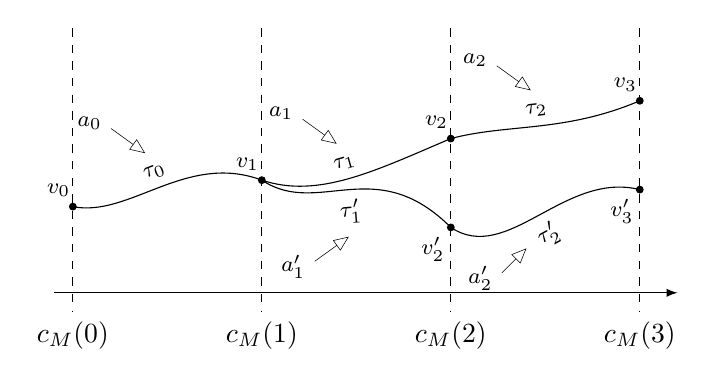
\begin{tikzpicture}[scale=2.4]
%baseline
\draw[-latex,thin] (-0.1,0) -- (3.2,0);
\foreach \x in {0,1,2,3}
\draw[shift={(\x,0)},thin,dashed] (0,1.4) -- (0,-0.1) node[below] { $c_M(\x)$};
%curves
\begin{scope}[yshift=7pt,font=\footnotesize]
\filldraw (0,0.21) circle (0.5pt) node[above,xshift=-1.2ex] {$v_0$};
\draw (0,0.21) .. controls (0.3,0.15) and (0.6,0.5) .. node[above,sloped] (t0) {$\tau_0$} (1,0.35);
\draw[-open triangle 45,very thin] ($(t0.north) + (-0.2,0.15)$) node[left,yshift=2pt] {$a_0$} -- ($(t0.north) + (-0.02,0.02)$);
	\filldraw (1,0.35) circle (0.5pt) node[above,xshift=-1.2ex] {$v_1$};
	\draw (1,0.35) .. controls (1.3,0.25) and (1.6,0.4) .. node[above,sloped] (t1) {$\tau_1$} (2,0.57);
	\draw[-open triangle 45,very thin] ($(t1.north) + (-0.2,0.15)$) node[left,yshift=2pt] {$a_1$} -- ($(t1.north) + (-0.02,0.02)$);
		\filldraw (2,0.57) circle (0.5pt) node[above,xshift=-1.2ex] {$v_2$};
		\draw (2,0.57) .. controls (2.3,0.65) and (2.6,0.6) .. node[above,sloped] (t2) {$\tau_2$} (3,0.77);
		\draw[-open triangle 45,very thin] ($(t2.north) + (-0.2,0.15)$) node[left,yshift=2pt] {$a_2$} -- ($(t2.north) + (-0.02,0.02)$);
			\filldraw (3,0.77) circle (0.5pt) node[above,xshift=-1.2ex] {$v_3$};
	\draw (1,0.35) .. controls (1.3,0.15) and (1.6,0.5) .. node[below,sloped] (t1') {$\tau_1'$} (2,0.1);
	\draw[-open triangle 45,very thin] ($(t1'.south) + (-0.2,-0.15)$) node[left,yshift=-2pt] {$a_1'$} -- ($(t1'.south) + (-0.02,-0.02)$);
		\filldraw (2,0.1) circle (0.5pt) node[below,xshift=-1.5ex] {$v_2'$};
		\draw (2,0.1) .. controls (2.3,-0.1) and (2.6,0.4) .. node[below,sloped] (t2'){$\tau_2'$} (3,0.3);
		\draw[-open triangle 45,very thin] ($(t2'.west) + (-0.15,-0.15)$) node[left,yshift=-2pt] {$a_2'$} -- ($(t2'.west) + (-0.02,-0.02)$);
			\filldraw (3,0.3) circle (0.5pt) node[below,xshift=-1.5ex] {$v_3'$};;;
\end{scope}
\end{tikzpicture}
\caption{A periodic dynamic system $E_M$.
%where
%$((a_0,v_0), \tau_0) \in \Lambda$, 
%$((a_1,v_1), \tau_1) \in \Lambda$, 
%$((a_1',v_1), \tau_1') \in \Lambda$, etc.
%$((a_2,v_2), \tau_2) \in \Lambda$, 
%$((a_2',v_2), \tau_2') \in \Lambda$, 
%and so on.
}
\label{fig:physical-transition}
\end{figure}





A controller machine $M = (D_i, S, D_o,\delta_{M})$ is considered as 
a \emph{nondeterministic} typed
machine that is
parameterized  by any possible \emph{observable}
behavior of its physical environment $E_M  = (C, P, U, \Lambda)$.%
\footnote{A controller $M$
is assumed to be tightly integrated with its physical environment 
$E_M$,
and thus $M$ can observe or affect $E_M$  immediately;
for ``remote'' sensors and actuators, % not tightly integrated,
they  can be considered as parts of another
controller that communicates with $M$ via a network \cite{ftscs-journal}.}
Each state $s \in S$ of $M$ provides:
%
\begin{inparaenum}[(i)]
	\item the current control command %of $M$ 
	to $E_M$,
	denoted by $\pi_C(s) \in C$,
	\item 
	the ``observed'' physical state by $M$
	from a physical state  $\vec{v} \in P$ of $E_M$,
	denoted by $\pi_P(s) = \pi_O(\vec{v})$, and
	\item the current local time of $M$,
	denoted by $\pi_t(s) \in \mathbb{N}$.
\end{inparaenum}
%
Notice that the ``observed'' physical parameters of $E_M$  are 
also parts of $M$'s (discrete) state,
and the control commands to $E_M$ are given based on the current state of $M$.

The \emph{environment restriction} of $M$ %by $E_M$ 
is the typed machine
$M \restriction E_M = (D_i, S \times P, D_o, \delta_{M \restriction E_M})$,
where its transition $\delta_{M \restriction E_M}$ is constrained by the observed behavior of $E_M$. That is,
%
$( (\vec{d}_i, (s,\vec{v})), ((s',\pvec{v}'), \vec{d}_o) ) \in \delta_{M \restriction E_M}$
iff:

\begin{itemize}
	\item $( (\vec{d}_i, s), (s', \vec{d}_o) ) \in \delta_{M}$,
	and $\pi_t(s') = \pi_t(s) + 1$,
	
	\item $\pi_P(s) = \pi_O(\vec{v})$, and $\pi_P(s') = \pi_O(\pvec{v}')$, and
	
	\item from the current physical state $\vec{v}$ at time $c_M(\pi_t(s))$,
	%where $\pi_P(s) = \pi_O(\vec{v})$,
	the ``next'' physical state $\pvec{v}'$ at time $c_M(\pi_t(s'))$
	%where $\pi_P(s') = \pi_O(\pvec{v}')$,
	is reachable 
	through some trajectory $\vec{\tau}$ %\in \mathcal{T}^l
	of  $E_M$ based on the current control command $\pi_C(s)$.
		Formally:
	\begin{alignat*}{3}
	((\pi_C(s), \vec{v}),  \vec{\tau} ) \in \Lambda,
	\quad&
	\vec{\tau}(0) = \vec{v},
	\\
	\quad&
	\vec{\tau}(c_M(\pi_t(s')) - c_M(\pi_t(s))) = \pvec{v}'.
	\end{alignat*}
\end{itemize}

\noindent
This extends the notion of environment restrictions in \cite{ftscs-journal},
which is a special case when $M$'s local clock is exactly the same as the global clock
(i.e., $c_M(n) = nT$ for $n \in \mathbb{N}$).





A physical correlation between $N$ physical environments 
$E_{M_i} = (C_i, P_i, c_{M_i}, \Lambda_i)$ 
for $i \in \{1, 2, \ldots, N\}$
can be specified by  a \emph{time-invariant constraint}
\[
(\forall t)\; \psi(\vec{x}_1(t), \vec{x}_2(t), \ldots, \vec{x}_N(t))
\]
over $E_{M_i}$'s parameters $\vec{x}_i$,
where $\psi$ is a logic formula over real numbers
with extra function symbols $\vec{x}_1, \ldots, \vec{x}_N$
yet \emph{no} free variables
(the parameters $\vec{x}_1, \ldots, \vec{x}_N$ are considered as trajectories).
%
A tuple of  trajectories 
$(\vec{\tau}_1, \vec{\tau}_2, \ldots, \vec{\tau}_N)$ 
of the parameters $\vec{x}_1, \ldots, \vec{x}_N$
is \emph{realizable} up to time $X \in \mathbb{R}_{\geq 0}$
iff 
$\psi(\vec{\tau}_1(t), \vec{\tau}_2(t), \ldots, \vec{\tau}_N(t))$
holds for every $t \in [0, X]$.
To verify a system design $\mathcal{E}$ 
where its subcomponents may have their local physical environments,
we examine every behavior of $\mathcal{E}$
given by realizable trajectories in Section~\ref{sec:dcps-bmc}.








In principle, a time-invariant constraint $\psi$ can be any first order logic formula,
but %in this paper 
we focus on \emph{equality} constraints
in which equalities are only predicate symbols.
In practice, many physical correlations can  be captured by
using such equality
constraints
as illustrated by examples in this paper.
%
For instance, if a parameter $x_1$ of $E_{M_1}$
must be equal to a parameter $x_2$ of $E_{M_2}$,
then the time-invariant constraint is given by $(\forall t)\; x_1(t) = x_2(t)$.
In this case,
the behavior of $E_{M_1}$ can immediately affect 
 $E_{M_2}$ using the parameter $x_1$.


 
\subsection{Example}
\label{sec:thermo-example}

We consider two simple hybrid systems to illustrate our approach.
Figure~\ref{fig:thermostat} shows a thermostat controller with a local clock,
adapted from \cite{hybridaut,ftscs-journal},
operating at a certain rate to control a temperature, 
specified by the typed machine
\[
M = (\mathbb{R}^2, \{m_\texttt{on},m_\texttt{off}\} \times \mathbb{N} \times \mathbb{R}, \{\ast\}, \delta_M).
\]
For each step, %the controller 
$M$ receives two inputs 
$(t_{\max},t_{\min}) \in \mathbb{R}^2$
from other controllers,
which denote the desired maximum and minimum temperature, respectively.
Each state $(m, n, v)$
is a tuple of a heater's mode $m \in \{m_\texttt{on},m_\texttt{off}\}$,
a counter $n$ to denote time $c_M(n)$ at the beginning of the current period, and
an observed temperature $v \in \mathbb{R}$ at time $c_M(n)$.
%
The output set $\{\ast\}$ indicates that $M$ has no output port.
The transition relation $\delta_M$
defines the next state $(m', n + 1, v')$ from
input $(t_{\max},t_{\min})$ and a state $(m, n, v)$, where:
\[\begin{medsize}
\begin{alignedat}{3}
(( (t_{\max},t_{\min}), (m_\texttt{on},n,v))&, ((m_\texttt{on}, n+1, v'),\ast)) &\in \delta_M	&\quad\mbox{if}\;\;	v \leq t_{\max} 
\\
(( (t_{\max},t_{\min}), (m_\texttt{on},n,v))&, ((m_\texttt{off}, n+1, v'),\ast)) &\ \in \delta_M	&\quad\mbox{if}\;\;	v > t_{\max} 
\\
(( (t_{\max},t_{\min}), (m_\texttt{off},n,v))&, ((m_\texttt{on}, n+1, v'),\ast)) &\in \delta_M	&\quad\mbox{if}\;\;	v <  t_{\min} 
\\
(( (t_{\max},t_{\min}), (m_\texttt{off},n,v))&, ((m_\texttt{off}, n+1, v'),\ast)) &\in \delta_M	&\quad\mbox{if}\;\;	v \geq t_{\min}.
\end{alignedat}
\end{medsize}\]
The \emph{next} observed temperature $v' \in \mathbb{R}$ 
at time $c_M(n+1)$ %the beginning of the \emph{next} period
can be any value, but  is determined by its physical environment $E_M$ below.
During each period, % (from $c_M(n)$ to $c_M(n + 1)$),
the controller $M$ gives a control command $\texttt{out}$ through its actuator
to turn the heater \emph{on}/\emph{off}
according to the mode $m \in \{m_\texttt{on},m_\texttt{off}\}$.



\begin{figure}
\centering
%layers to draw the block diagram
\pgfdeclarelayer{background}
\pgfdeclarelayer{foreground}
\pgfsetlayers{background,main,foreground}
\begin{tikzpicture}[scale=0.9] %baseline=-0.6ex
%states
\matrix[row sep=1ex,column sep=14ex,text centered]{
\node (on) [draw,circle,text width=4.6ex,font=\footnotesize] {$m_\texttt{on}$}; & 
\node (off) [draw,circle,text width=4.6ex,font=\footnotesize] {$m_\texttt{off}$};  \\
};
%text
\node[below,font=\scriptsize] at (on.south) {$\texttt{out} \leftarrow \mathit{on}$};
\node[below,font=\scriptsize] at (off.south) {$\texttt{out} \leftarrow \mathit{off}$};
%arrows
\path[->,font=\scriptsize]
(on) edge[bend left=40] node[above] {$v > t_{\max}$} (off)
(on) edge [loop left,in=150,out=-150,looseness=5] node[above=2ex] {$v \leq t_{\max}$} (on)
(off) edge[bend left=40] node[below] {$v< t_{\min}$} (on)
(off) edge [loop right,in=-30,out=30,looseness=5] node[above=2ex] {$v \geq t_{\min}$} (off);
%blocks
\begin{pgfonlayer}{background}
\path (on.west |- off.north)+(-1.5,0.9) node (a) {};
\path (off.east |- on.south)+(+1.5,-0.9) node (b) {};
\path[rounded corners, draw] (a) rectangle (b);
%ports
\draw [<-,thick] (on.west |- on.north)+(-1.3,0.2) -- node{ }+(-1.7,0.2) node[left] {$t_{\max}$};
\draw [<-,thick] (on.west |- on.south)+(-1.3,-0.2) -- node{ }+(-1.7,-0.2) node[left] {$t_{\min}$};
\draw [-open triangle 45,thick] (off.east |- off.north)+(1.3,0.2) -- node{ } + (1.7,0.2) node[right] {\texttt{out}};
\draw [open triangle 45-,thick] (off.east |- off.south)+(1.3,-0.2) -- node{ } + (1.7,-0.2) node[right] {$v$};
\end{pgfonlayer}
\end{tikzpicture}
%\quad
%$
%\dot{x} =
%\begin{cases}
%K (h - x) &\mbox{if } \texttt{out} = \mathit{on}\\
%- K x &\mbox{if } \texttt{out} = \mathit{off} 
%\end{cases}
%$
\caption{A digital thermostat controller \cite{ftscs-journal}.
%with two input ports $t_{\max}$ (a maximum temperature)
%and $t_{\min}$ (a minimum temperature).
}\label{fig:thermostat}
\end{figure}


%The physical environment EM of the nondeterministic digital thermostat controller M is specified by the 1-dimensional periodic dynamic system with period T:
%EM = ({on,off}, R, T, ?)
%with a set of control commands {on,off}, the physical state R for the current temperature x of the room,
%and the physical transition relation ? ? ({on, off } � R) � TT given by:

For the nondeterministic controller $M$,
its local physical environment $E_M$ models
the open room environment shown in Figure~\ref{fig:open-room},
where the temperature $x$ of the room changes 
based on the heater of $M$ and  the outside temperature $x_o$.
This environment $E_M$ is specified by:
\[
E_M = (\{\mathit{on},\mathit{off}\}, \mathbb{R}^2, T + 2\epsilon, \Lambda)
\]
for
a set of control commands $\{\mathit{on}, \mathit{off}\}$,
and 
a physical state $(v,v_o) \in \mathbb{R}^2$ 
to denote the room's temperature $x$ and the outside temperature $x_o$.
The physical transition relation 
$\Lambda$
% %\subseteq (\{\mathit{on},\mathit{off}\} \times \mathbb{R}^2) \times \mathcal{T}_{T+2\epsilon}^2$ 
is given by:
$
\big( (\texttt{out}, (v,v_o)), (\tau,\tau_o) \big) \in \Lambda
$
iff there are continuous trajectories $\tau, \tau_o: [0,T + 2\epsilon] \to \mathbb{R}$
for the parameters $x$ and $x_o$,
respectively, 
such that $\tau(0) = v$, $\tau_o(0) = v_o$, and:
\begin{equation}
\dot{x} =
\begin{cases}
K (h - ((1-k) x + k  x_o)) &\mbox{if } \texttt{out} = \mathit{on}\\
- K ((1-k) x + k  x_o) &\mbox{if } \texttt{out} = \mathit{off},
\end{cases}
\label{eq:open-thermo}
\end{equation}
where $K, h, k \in \mathbb{R}$ are constants depending on 
the size of the room, 
the power of the heater,
and the size of the door, respectively.
That is, given a \emph{nondeterministically chosen}
trajectory $\tau_o$ of the outside temperature $x_o$,
if the heater is on,
then the temperature $x$ rises according to the differential equation $\dot{x} = K (h - ((1-k) x + k  x_o))$,
and if the heater is off,
then 
the temperature $x$ falls according to the differential equation $\dot{x} = - K ((1-k) x + k  x_o)$.
 
\begin{figure}
\centering
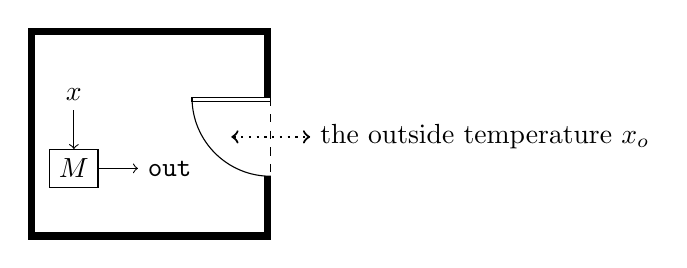
\begin{tikzpicture}[scale=1.00]
%room
\filldraw (0,-1.2) rectangle  + (-0.08,0.8)
	(0,-0.4) rectangle  + (-3,0.08)
	(-3,-0.32) rectangle  + (-0.08,-2.6)
	(-3.08,-3.0) rectangle  + (3,0.08)
	(0,-3.0) rectangle  + (-0.08,0.8);
%M
\path (-2.5,-2.1) node[draw] (machine) { $M$};
\draw[<-] (machine.north) -- node {} + (0,0.5) node[above] {$x$};
\draw[->] (machine.east) -- node {} + (0.5,0) node[right] {$\texttt{out}$};
%door
\draw[dashed] (0,-1.2) -- (0,-2.2);
\draw (0,-1.2) rectangle +(-1,-0.05);
\draw (-1,-1.2) arc (180:270:1);
%outside
\draw[<->,dotted,thick] (-0.5,-1.7) -- (0.5,-1.7) node[right] {the outside temperature $x_o$};
\end{tikzpicture}
\caption{Open room environment.
%with two input ports $t_{\max}$ (a maximum temperature)
%and $t_{\min}$ (a minimum temperature).
}\label{fig:open-room}
\end{figure}

By definition, the environment restriction of $M$ by $E_M$ 
is the typed machine 
$M \restriction E_M = (\mathbb{R}^2, S \times P, \{\ast\}, \delta_{M \restriction E_M})$
with
$M$'s state space $S = \{m_\texttt{on},m_\texttt{off}\} \times \mathbb{N} \times \mathbb{R}$
and $E_M$'s physical state space $P = \mathbb{R}^2$.
The combined transition
$(( (t_{M},t_{m}), (m,n,v,v,v_o)),\,
 ((m',n',v', v',v_o'),\ast)) \in \delta_{M \restriction E_M}$
of the machine $M \restriction E_M$
holds iff:

\begin{itemize}
	\item $(( (t_{M},t_{m}), (m,n,v)), ((m',n',v'),\ast)) \in \delta_M$ (i.e., 
	the $M$'s transition holds) with $n' = n + 1$,
	where
	 $M$'s periodic local time is given by $\pi_t(m, n, v) = n$;

	\item the observed physical parameters of $E_M$ are given by
	$\pi_P(m,n,v) = v$ and
	$\pi_O(v,v_o) = v$;
	and
	\item there are $E_M$'s trajectories $(\tau, \tau_o) \in \mathcal{T}_{T+2\epsilon}^2$
	 % of duration $T + 2\epsilon$
	 such that
	 \begin{align*}
	 ((\pi_C(m,n,v), (v,v_o)),  (\tau,\tau_o) ) &\in \Lambda, \\
	 (\tau,\tau_o)(0) &= (v,v_o), \\
	 (\tau,\tau_o)(c_M(n+1) - c_M(n)) &= (v',v_o'),
	 \end{align*}
	 where $M$'s control commands to $E_M$ are defined by
	 $\pi_C(m_\texttt{on}, n, v) = \mathit{on}$ and $\pi_C(m_\texttt{off}, n, v) = \mathit{off}$.
\end{itemize}

\noindent
For example,
given a \emph{constant} outside temperature ($\dot{x_o} = 0$),
the combined behavior of %the environment restriction 
$M \restriction E_M$
is shown in Figure~\ref{fig:restriction-diagram-thermo}.
From a physical state $\vec{v}_i$ at time $c_M(i)$,
the next \emph{observed} physical state $\vec{v}_{i+1}$ 
(at time $c_M(i+1)$)
is given according to  
the differential equations~(\ref{eq:open-thermo}) and $\dot{x_o} = 0$. 





\begin{figure}
\centering
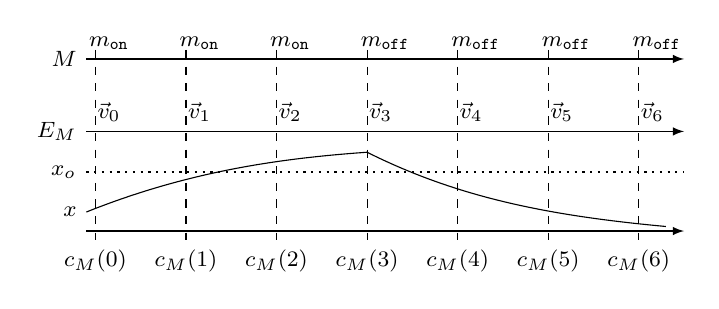
\begin{tikzpicture}[scale=1.15,font=\footnotesize]
%baseline
\draw[-latex,thin] (-0.1,0) node[left] {% Step
}-- (6.5,0);
%\draw[shift={(0,0)},thin] (0,1.9) -- (0,-0.1);
\foreach \x in {0,1,2,3,4,5,6}
\draw[shift={(\x,0)},thin,dashed] (0,2.0) -- (0,-0.1) node[below] { $c_M(\x)$};
%M_{E_M}              
\draw[-latex,thin] (-0.1,1.1) node[left] { $E_M$} -- (6.5,1.1);
\foreach \z in {0,1,2,3,4,5,6}
\path (\z+0.15,1.1) node[above] { $\vec{v}_\z$};
%M
\draw[-latex,thin] (-0.1,1.9) node[left] { $M$} -- (6.5,1.9);
\foreach \z in {1,2,3} \path (\z-0.85,1.9)  node[above] {$m_{\texttt{on}}$};
\foreach \z in {4,5,6,7} \path (\z-0.8,1.9)  node[above] {$m_{\texttt{off}}$};
%x_0 line
\draw[thick,dotted] (-0.1,0.65) node[left] { $x_o$} -- (6.5,0.65);
%x curves
\draw (-0.1,0.21) node[left] { $x$} .. controls (1,0.65) and (2,0.8) .. (3,0.87);
%\draw[shift={(0,-0.15)},smooth,samples=1000,domain=-0.1:3] plot(\x,{1.2-0.8*exp(-0.5*\x)});
\draw (3,0.87) .. controls (4,0.37) and (5,0.17) .. (6.3,0.05);
%\draw[shift={(0,-0.15)},smooth,samples=1000,domain=3:6.3] plot(\x,{4.58*exp(-0.5*\x)});
%
\end{tikzpicture}
\caption{The behavior of $M \restriction E_M$,
when $\dot{x_o} = 0$.
%the digital thermostat controller $M$ with period $T$
%integrated with its physical environment $E_M$.
}
\label{fig:restriction-diagram-thermo}
\end{figure}


We now consider digital thermostat controllers 
$M_1$ and $M_2$ that are 
respectively installed in two \emph{adjacent} rooms connected by an open 
door, as illustrated in Figure~\ref{fig:adj-rooms}.
The temperature of each room is separately controlled by 
the normal thermostat controller in Figure~\ref{fig:thermostat}
that turns on/off the switch of the heater in the room:
for $i=1,2$,
\[
M_i = (\mathbb{R}^2, \{m_\texttt{on},m_\texttt{off}\} \times \mathbb{N} \times \mathbb{R}, \{\ast\}, \delta_{M_i}).
\]
Suppose that $M_1$ and $M_2$ have different rates. For example,
$\mathit{rate}(1) = 2$ and $\mathit{rate}(2) = 3$;
i.e., for the logical periods $T_1$ and $T_2$ of $M_1$ and $M_2$, respectively,
$2 T_1 = 3 T_2$ holds.


The local physical environment $E_{M_i}$ of each controller $M_i$
can be just considered as the open room environment in Figure~\ref{fig:open-room}
explained above.
That is, for $i = 1,2$:
\[
E_{M_i} = (\{\mathit{on},\mathit{off}\}, \mathbb{R}^2, T_i + 2\epsilon, \Lambda_i).
\]
Similarly,
the physical transition relation $\Lambda_i$ %for $i = 1,2$
states that 
the room's temperature $x_i$  and the outside temperature $x_{o_i}$
are  governed by the following differential equation:
\[
\dot{x}_i =
\begin{cases}
K_i (h_i - ((1-k) x_i + k  x_{o_i})) &\mbox{if } \texttt{out}_i = \mathit{on}\\
- K_i ((1-k) x_i + k  x_{o_i}) &\mbox{if } \texttt{out}_i = \mathit{off}.
\end{cases}
\]
where $K_i, h_i \in \mathbb{R}$ are constants given by the size of each room
and the heater's power, respectively,
and $k \in \mathbb{R}$ is a constant based on the size of the open door. 
Recall that 
the behavior of each $E_{M_i}$ depends on 
\emph{nondeterministic chosen} trajectories of 
the outside temperature $x_{o_i}$.

\begin{figure}
\centering
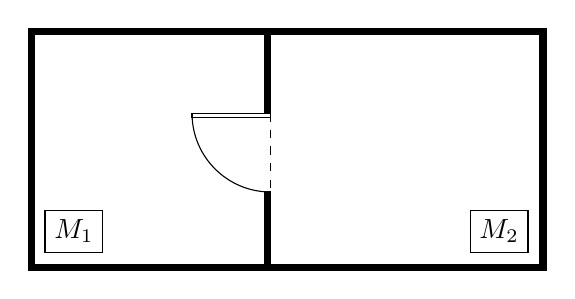
\begin{tikzpicture}[baseline=(current bounding box.north)]
%room1
\filldraw (0,-1) rectangle  + (-0.08,1)
	(0,0) rectangle  + (-3,0.08)
	(-3,0.08) rectangle  + (-0.08,-3)
	(-3.08,-3) rectangle  + (3,0.08)
	(0,-3) rectangle  + (-0.08,1);
\path (-2.5,-2.5) node[draw] { $M_1$};
\draw[dashed] (0,-1) -- (0,-2);
%room2
\filldraw (0,0) rectangle  + (3.5,0.08)
	(3.5,0.08) rectangle  + (-0.08,-3)
	(3.5,-3) rectangle  + (-3.5,0.08);
\path (2.9,-2.5) node[draw] (m2){ $M_2$};
%door
\draw (0,-1) rectangle +(-1,-0.05);
\draw (-1,-1) arc (180:270:1);
\end{tikzpicture}
\caption{Two rooms connected by an open door.
} \label{fig:adj-rooms}
\end{figure}



However,
because those two rooms $1$ and $2$ are physically connected %to each other 
by the open door,
the outside temperature $x_{o_1}$ of the room~$1$
must be equal to
the temperature $x_2$ of the room~$2$, and vice versa.
This can be precisely specified by the time-invariant constraint between $E_{M_1}$ and $E_{M_2}$:
\begin{equation}
(\forall t)\;
x_{o_1}(t) = x_2(t)
\;\wedge\;
x_{o_2}(t) = x_1(t).
\label{eq:thermo-connected}
\end{equation}
By adding this constraint,
the composed behavior of
the nondeterministic physical environments 
$E_{M_1}$ and $E_{M_2}$ 
is now \emph{deterministic},
since the outside temperature $x_{o_i}$ of each $E_{M_i}$
is determined by the temperature of the other room.


Figure~\ref{fig:room-ensemble}
shows a multirate ensemble $\mathcal{E}$
for controlling the temperatures of the two adjacent rooms.
the ensemble $\mathcal{E}$ consists of 
three discrete components:
The main controller $\mathtt{Main}$
sets a maximum temperature $t_{\max}$ and  a minimum temperature $t_{\min}$ for both
of the rooms,
and
each thermostat controller $M_i$ ($i = 1,2$) then controls the room's heather
according to given $t_{\max}$ and $t_{\min}$.
Because the behavior of each controller $M_i$ is restricted by 
the behavior of its local physical environment $E_{M_i}$,
the machine in the ensemble $\mathcal{E}$ is indeed
the environment restriction $M_i \restriction E_{M_i}$,
which further satisfies 
the time-invariant constraint (\ref{eq:thermo-connected}).
Notice that the behavior of each $M_i \restriction E_{M_i}$
is also parameterized by the exact local clock $c_{M_i}$ of each controller $M_i$,
since $M_i$ ``observes'' the current temperature
based on $c_{M_i}$.



\begin{figure}
\centering
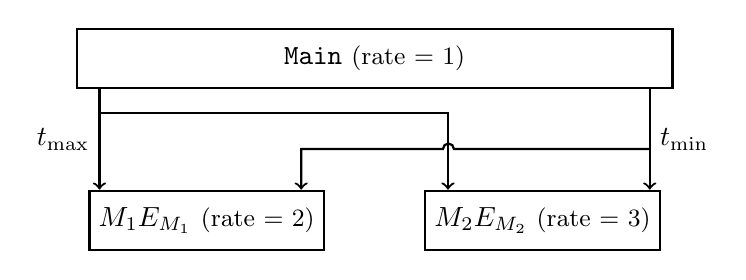
\begin{tikzpicture} %[baseline=(current bounding box.north)]
\node (main) [draw,thick,minimum width=50ex,minimum height=5ex] 
{$\mathtt{Main}$ {\small (rate = 1)}}; % 
\path (main.west |- main.south) + (11ex,-11ex) node (t1) [draw,thick,minimum width=16ex,minimum height=5ex] 
{$M_1\restriction E_{M_1}$ {\small (rate = 2)}}; %
\path (main.east |- main.south) + (-11ex,-11ex) node (t2) [draw,thick,minimum width=16ex,minimum height=5ex] 
{$M_2\restriction E_{M_2}$ {\small (rate = 3)}}; %
%connection t_max
\draw [thick,->] ($(main.west |- main.south)+(2ex,0)$) 
	-- node[left] {$t_{\max}$} ($(main.west |- t1.north) + (2ex,0)$);
\draw [thick,->] ($(main.west |- main.south)+(2ex,-2ex)$) 
	-- node {} ($(t2.west |- main.south) + (2ex,-2ex)$) 
	-- node {} ($(t2.west |- t2.north) + (2ex,0)$);
%connection t_min
\draw [thick,->] ($(main.east |- main.south)+(-2ex,0)$) 
	-- node[right] {$t_{\min}$} ($(main.east |- t2.north) + (-2ex,0)$);
\draw [thick,->] ($(main.east |- main.south)+(-2ex,-5ex)$) 
	-- ($(t2.west |- main.south) + (2.5ex,-5ex)$) arc(0:180:.7mm)
	-- node {} ($(t1.east |- main.south) + (-2ex,-5ex)$) 
	-- node {} ($(t1.east |- t1.north) + (-2ex,0)$);
%ports
%\draw [<-,thick] (t1.west |- t1.south) + (2ex,0)-- node{ }+(2ex,-2ex) node[below] {$x_1$};
%\draw [->,thick] (t1.east |- t1.south) + (-2ex,0)-- node{ }+(-2ex,-2ex) node[below] {$\texttt{out}_1$};
%\draw [<-,thick] (t2.west |- t2.south) + (2ex,0)-- node{ }+(2ex,-2ex) node[below] {$x_2$};
%\draw [->,thick] (t2.east |- t2.south) + (-2ex,0)-- node{ }+(-2ex,-2ex) node[below] {$\texttt{out}_2$};
\end{tikzpicture}
\[
(\forall t)\;
x_{o_1}(t) = x_2(t)
\;\wedge\;
x_{o_2}(t) = x_1(t).
\vspace{-0.7ex}
\]
\caption{A multirate ensemble $\mathcal{E}$} \label{fig:room-ensemble}
\end{figure}



%
\section{SMT-based Model Checking}
\label{sec:dcps-bmc}

A distributed CPS specified 
by the modeling framework in Section~\ref{sec:dcps-design},
using multirate ensembles, periodic dynamic systems,
and time-invariant constraints,
can be verified by simulating all possible behavior of the system,
provided that the \emph{concrete} parameters (e.g., inputs and exact local clocks) are given.
For example, 
the previous execution framework in \cite{ftscs-journal}---that
assumes no time-invariant constraints and no local clock skews---can 
be easily adapted  for this purpose.
In this case, 
we can verify the system with respect to
a \emph{finite} number of (specified) parameters for the system.

However, 
the system may in general involve an \emph{infinite} number of 
(real number) parameters. % and inputs.
For example, 
in the distributed thermostat controller of Section~\ref{sec:thermo-example},
it is more realistic to assume that 
the main controller can give
the outputs $(t_{\max}, t_{\min})$
from  any reals within certain bounds,
rather than from a finite set of specified reals.
Also, 
exact values of local clocks %for distributed components 
in the system 
is determined on-the-fly by 
\emph{clock synchronization} mechanisms \cite{pals-rtss09,lynch-book}.
It is in practice not possible to 
predict such an exact local clock $c_M$ of a controller $M$,
since there are infinitely many possibilities for $c_M$.
Consequently, 
model checking by explicitly simulating the system
is not satisfactory for CPS, %in general,
because it is not possible to simulate it
for every parameter. 

This section explains how we can verify the system 
even for such an infinite number of  parameters, inputs, and local clocks.
Instead of explicitly simulating the system as usual,
we \emph{symbolically} represent the behavior of the system
as logic formulas
up to a given bound,
where the safety requirements %of the system 
are also expressed as certain logic formulas
(Section~\ref{sec:formula}).
Then, we verify the system %up to any given precision $\delta > 0$
by checking the satisfiability of these formulas
%using $\delta$-complete SMT solving 
using the \texttt{dReal} SMT solver (Section~\ref{sec:component-dReal}).
%This also involves a nontrivial extension of  \texttt{dReal},
%since, due to the distributed nature of the system,
%the generated formula may include uninterpreted real function symbols
%that are not supported by the existing \texttt{dReal} interface.
Our approach is illustrated with the distributed thermostat example,
and later with the case studies in Section~\ref{sec:case-studies}.

 



\subsection{Generating Logic Formulas}
\label{sec:formula}

For a machine  $M = (D_i,S,D_o,\delta_M)$
with $n$ input ports and $m$ output ports,
its transition $\delta_M \subseteq (D_i \times S) \times (S \times D_o)$
can be naturally expressed as a %first order 
logic formula of the form:
\[
\varphi_{M}(y_{i_1},\ldots,y_{i_n}\shortmid
y_{s_1},\ldots,y_{s_k}\shortmid
y_{s_1}',\ldots,y_{s_k}'\shortmid
y_{o_1},\ldots,y_{o_m}),
\]
with:
\begin{inparaenum}[(i)]
	\item the variables $y_{i_1},\ldots,y_{i_n}$ for the inputs,
	\item the variables $y_{s_1},\ldots,y_{s_k}$  for the current discrete state, 
	\item the variables $y_{s_1}',\ldots,y_{s_k}'$  for the next discrete state, and 
	\item the variables $y_{o_1},\ldots,y_{o_m}$  for the outputs.
\end{inparaenum}
That is:
\begin{equation}
\varphi_{M}(\vec{d}_i\shortmid s\shortmid s'\shortmid  \vec{d}_o)
\;\iff\;
( (\vec{d}_i, s), (s', \vec{d}_o) ) \in \delta_{M}
\label{eq:formula-rel-machine}
\end{equation}
In practice, the transitions of a controller are written 
in a modeling language (such as C),
and the logic of the controller in the language
is directly translated into the formula $\varphi_{M}$.


\begin{example}
\label{ex:thermo-formula}
Consider the digital thermostat controller in Figure~\ref{fig:thermostat},
given by
$M = (\mathbb{R}^2, \{m_\texttt{on},m_\texttt{off}\} \times \mathbb{N} \times \mathbb{R}, \{\ast\}, \delta_M)$.
The logic formula $\varphi_{M}$ can be expressed by:
\begin{alignat*}{2}
&
\varphi_{M}(
y_{t_{\max}}, y_{t_{\min}}\shortmid
y_m, y_n, y_v\shortmid
y_m', y_n', y_v'\shortmid
\ast)
\\
\ArrowBetweenLines[\equiv]
%
& y_n' = y_n + 1 \;\wedge\; 
\\
& 
\left(
\begin{aligned}
&(y_m = m_\texttt{on} \;\wedge\; y_v \leq y_{t_{\max}} \;\wedge\; y_m' = m_\texttt{on}) \;\vee\;
\\
& (y_m = m_\texttt{on} \;\wedge\; y_v > y_{t_{\max}} \;\wedge\; y_m' = m_\texttt{off}) \;\vee\;
\\
& (y_m = m_\texttt{off} \;\wedge\; y_v < y_{t_{\min}} \;\wedge\; y_m' = m_\texttt{on}) \;\vee\;
\\
& (y_m = m_\texttt{off} \;\wedge\; y_v \geq y_{t_{\min}} \;\wedge\; y_m' = m_\texttt{on})
\end{aligned}
\right)
\end{alignat*}
\end{example}


%Similarly, 
For a $U$-periodic dynamic system
$E_M = (C, P, U, \Lambda)$,
its physical transition relation
$\Lambda$ can be expressed as a first order formula
over reals of the form:
\[
\varphi_{E_M}(
y_{C_1},\ldots,y_{C_j}\shortmid
y_{v_1}, \ldots, y_{v_l}\shortmid
x_1, \ldots, x_l\shortmid
y_t, y_t'
)
\]
with:
\begin{inparaenum}[(i)]
	\item the variables $y_{C_1},\ldots,y_{C_j}$  for control commands  from $M$,
	\item the variables $y_{v_1}, \ldots, y_{v_l}$  for the initial values 
	of $E_M$'s physical parameters $x_1, \ldots, x_l$, 
	\item the unary \emph{function symbols} $x_1, \ldots, x_l$
	denoting $E_M$'s physical parameters,
	and
	\item  the variables $y_t$ and $y_t'$ denoting times 
	at the beginning and the end of the period, respectively.
\end{inparaenum}
%
The formula $\varphi_{E_M}$ defines 
the trajectories of the physical parameter $x_1, \ldots, x_l$ %of duration $y_t' - y_t$
during the time interval  $[y_t, y_t']$. 
%after time $y_t' - y_t$ elapsed.
That is,
\begin{equation}
\begin{aligned}
&
\varphi_{E_M}(a\shortmid \vec{v}\shortmid \vec{x}\shortmid y_t, y_t')
\\
\iff\;\;
&
((a, \vec{v}),  \vec{\tau}) \in \Lambda
\;\wedge\;
\forall t \in [y_t, y_t'].\; \vec{x}(t) = \vec{\tau}(t - y_t)
\end{aligned}
\label{eq:formula-rel-env}
\end{equation}
The solution functions for differential equations
are written in the formula $\varphi_{E_M}$
by using integral operators.


\begin{example}
\label{ex:openroom-formula}
Consider the open room local environment of 
the thermostat controller $M$
in Section~\ref{sec:thermo-example}, given by
the periodic dynamic system
$E_M = (\{\mathit{on},\mathit{off}\}, \mathbb{R}^2, T + 2\epsilon, \Lambda)$.
The logic formula $\varphi_{E_M}$ can be expressed by:
\begin{alignat*}{2}
&
\varphi_{E_M}(y_{\texttt{out}}\shortmid y_v, y_{v_o}\shortmid x, x_o\shortmid  y_t,y_t')
\\
\ArrowBetweenLines[\equiv]
& 
x_o(y_t) = y_{v_o} \;\wedge\; 
\\
&
\left(
\begin{aligned}
(y_{\texttt{out}} = \mathit{on}
&\;\wedge\; 
\forall t \in [y_t,y_t'].\; x(t) = \mathit{flow}_{\!\mathit{on}}(y_v, t)) \;\vee\;
\\
(y_{\texttt{out}} = \mathit{off}
&\;\wedge\; 
\forall t \in [y_t,y_t'].\; x(t) = \mathit{flow}_{\!\mathit{off}}(y_v, t))
\end{aligned}
\right)
\end{alignat*}
where
$\mathit{flow}_{\!\mathit{on}}(y_v, t) = y_v + \int_{y_t}^{t} K (h - ((1-k) x + k  x_o)) \,\mathrm{d} t$
and
$\mathit{flow}_{\!\mathit{off}}(t) = y_v + \int_{y_t}^{t} (- K ((1-k) x + k  x_o)) \,\mathrm{d} t$.
The parameters $x$ and $x_o$ in the formula $\varphi_{E_M}$
are \emph{not} variables,
but \emph{logical operators} to denote unary functions 
$x, x_o: \mathbb{R} \to \mathbb{R}$.
% over reals.
\end{example}



Now consider the \emph{environment restriction} of $M$ by $E_M$,
namely,
$M \restriction E_M = (D_i, S \times P, D_o, \delta_{M \restriction E_M})$.
The combined transition relation $\delta_{M \restriction E_M}$
can then be expressed as a logic formula
in a straightforward way as follows:

\begin{align*}
&
\varphi_{M \restriction E_M}(\vec{y}_i\shortmid \vec{y}_s,\; \vec{y}_v\shortmid \pvec{y}_{\!s}',\; \pvec{y}_{\!v}'\shortmid \vec{y}_o)
\\
\ArrowBetweenLines[\equiv]
&
\varphi_M(\vec{y}_i\shortmid \vec{y}_s\shortmid \pvec{y}_{\!s}'\shortmid \vec{y}_o)
\;\wedge\;
\pi_t(\pvec{y}_{\!s}') = \pi_t(\vec{y}_s) + 1
\;\wedge
\\
&
\pi_P(\vec{y}_s) = \pi_O(\vec{y}_v) 
\,\;\quad\wedge\; \pi_P(\pvec{y}_{\!s}') = \pi_O(\pvec{y}_{\!v}')
\;\wedge
\\
&
\varphi_{E_M}( \pi_C(\vec{y}_s)\shortmid \vec{y}_v\shortmid \vec{x}\shortmid \pi_t(\vec{y}_{s}), \pi_t(\pvec{y}_{\!s}'))
\;\wedge
\\
&
\vec{y}_{v} = \vec{x}(c_M(\pi_t(\vec{y}_{s})))
\,\,\wedge\;
\pvec{y}_{\!v}' = \vec{x}(c_M(\pi_t(\pvec{y}_{\!s}'))),
\end{align*}
%
where the four projection functions  $\pi_t$,  $\pi_P$, $\pi_O$, and $\pi_C$
are defined for tuples of variables in an expected way.
Notice that the definition of $\varphi_{M \restriction E_M}$
is just a direct translation of the definition of $\delta_{M \restriction E_M}$
in Section~\ref{sec:env-const}
with the equivalences (\ref{eq:formula-rel-machine}) and (\ref{eq:formula-rel-env}),
which implies the equivalence:
\begin{equation}
\begin{aligned}
&
\varphi_{M \restriction E_M}(\vec{d}_i\shortmid s,\, \vec{v} \shortmid s',\, \pvec{v}' \shortmid \vec{d}_o)
\\
\iff\quad&
( (\vec{d}_i, (s,\vec{v})), ((s',\pvec{v}'), \vec{d}_o) ) \in \delta_{M \restriction E_M}
\end{aligned}
\end{equation}

\begin{example}
Consider the environment restriction 
of the thermostat controller $M$ by the open room environment $E_M$
in Section~\ref{sec:thermo-example},
given by
$M \restriction E_M = (\mathbb{R}^2, S \times P, \{\ast\}, \delta_{M \restriction E_M})$
with 
 $S = \{m_\texttt{on},m_\texttt{off}\} \times \mathbb{N} \times \mathbb{R}$
 and
$P = \mathbb{R}^2$.
The formula 
\[\varphi_{M \restriction E_M}(
y_{t_{M}}, y_{t_{m}}\shortmid
y_m, y_n, y_v, y_v, y_{v_o}\shortmid
y_m', y_n', y_v', y_v', y_{v_o}'\shortmid
\ast)\]
is defined 
using the formulas in 
Examples~\ref{ex:thermo-formula}--\ref{ex:openroom-formula}
as follows:
\begin{align*}
&
\varphi_{M}( y_{t_{M}}, y_{t_{m}}\shortmid y_m, y_n, y_v\shortmid y_m', y_n', y_v'\shortmid \ast) 
\;\wedge\;
y_n' = y_n + 1
\\
\wedge\;\;&
\varphi_{E_M}(y_m \shortmid y_v, y_{v_o}\shortmid x, x_o\shortmid  c_M(y_n),c_M(y_n'))
\\
\wedge\;\;&
y_v = x(c_M(y_n))
\;\wedge\;
y_{v_o} = x_o(c_M(y_n))
\\
\wedge\;\;&
y_v' = x(c_M(y_n'))
\;\wedge\;
y_{v_o}' = x_o(c_M(y_n'))
\end{align*}
where the projection functions are given by:
\begin{align*}
\pi_t(y_m, y_n, y_v) &= y_n,
&
\pi_P(y_m, y_n, y_v) &= y_v,
\\
\pi_O(y_v, y_{v_o}) &= y_v,
&
\pi_C(y_m, y_n, y_v) &= y_m.
\end{align*}
We can easily see that 
 $\varphi_{M \restriction E_M}$ is a direct translation of the 
definition of  $\delta_{M \restriction E_M}$
in Section~\ref{sec:thermo-example}.
\end{example}


To perform bounded model checking of a machine $M$,
we generate a logic formula
that expresses the behavior of $M$ up to $N$ steps
for a given bound $N \in \mathbb{N}$. 
Note that an environment restriction 
is also a typed machine, and thus treated in the same way
(see below for multirate ensembles and time-invariant constraints).
We can just \emph{symbolically execute}
transitions of $M$ to generate such a formula.
From given input variables $\vec{y}_{i}$ and state variables $\vec{y}_{s}$,
a \emph{symbolic transition function}  $\tilde{\delta}_M$ 
generates 
``next state'' variables $\pvec{y}_{\!s}'$,
output variables $\vec{y}_{o}$,
and the formula $\varphi_M(\vec{y}_i \shortmid \vec{y}_s \shortmid \pvec{y}_{\!s}' \shortmid \vec{y}_o)$
that defines the logical relations between the variables:
i.e.,
$\tilde{\delta}_M(\vec{y}_{i},  \vec{y}_{s}) = 
((\pvec{y}_{\!s}',\,
 \vec{y}_o),\,
\varphi_M(\vec{y}_i \shortmid \vec{y}_s \shortmid \pvec{y}_{\!s}' \shortmid \vec{y}_o))$,
where $\pvec{y}_{\!s}'$ and $\vec{y}_o$ are \emph{fresh new} variables.
Then,
a \emph{one-step formula generation process} for $M$ is straightforwardly defined as:
\begin{align*}
&
\langle\vec{y}_{s} \mid \mathcal{C} \rangle
\;\xrightarrow{\;\vec{y}_{i}\;}\;
\langle\pvec{y}_{\!s}' \mid
 \mathcal{C} \,\wedge\, \varphi_M(\vec{y}_i \shortmid \vec{y}_s \shortmid \pvec{y}_{\!s}' \shortmid \vec{y}_o)\rangle
\\
\iff\quad&
\tilde{\delta}_M(\vec{y}_{i},  \vec{y}_{s}) = 
((\pvec{y}_{\!s}',\,\vec{y}_o),\,
\varphi_M(\vec{y}_i \shortmid \vec{y}_s \shortmid \pvec{y}_{\!s}' \shortmid \vec{y}_o)),
\end{align*}
where $\mathcal{C}$ denotes the \emph{accumulated formula} generated in the previous steps.
We can perform 
this process for $N$ steps
from
the initial configuration 
$\langle\vec{y}_{s_0} \mid \varphi_{\mathit{Init}}(\vec{y}_{s_0}) \rangle$ 
with initial state variables $\vec{y}_{s_0}$
and an initial condition $\varphi_{\mathit{Init}}(\vec{y}_{s_0})$.






To generate a formula for  a multirate ensemble $\mathcal{E}$,
we can also symbolically execute
the synchronous composition of $\mathcal{E}$.
As explained in Section~\ref{sec:dcps-design},
each machine $M_j$ in $\mathcal{E}$
is already integrated with its local physical environment
(that is, $M_j$ is an environment restriction).
A symbolic transition function $\tilde{\delta}_{M_j}$ of each $M_j$
is well defined above:
given input variables $\vec{y}_{i_j}$ and state variables $\vec{y}_{s_j}$,
$\tilde{\delta}_{M_j}$ return 
next state variables $\pvec{y}_{\!s_j}'$,
output variables $\vec{y}_{o_j}$,
and the formula $\varphi_{M_j}$.
A symbolic transition function $\tilde{\delta}_\mathcal{E}$
of an ensemble $\mathcal{E}$
is then defined
by regarding such input/output variables 
$\vec{y}_{i_j}$ and $\vec{y}_{s_j}$
as normal data   in an obvious way.
A resulting formula $\varphi_{\mathcal{E}}$ of $\tilde{\delta}_\mathcal{E}$
is a conjunction of the formulas $\varphi_{M_j}$ for machines $M_j$
in $\mathcal{E}$,
plus a time-invariant $\varphi_{\mathit{INV}}$
for their local environments.
Then,
a one-step formula generation process for an ensemble $\mathcal{E}$
is defined by using $\tilde{\delta}_\mathcal{E}$
in the exactly same way.

More precisely, 
''symbolic states'' of an ensemble $\mathcal{E}$
consist of:
\begin{inparaenum}[(i)]
	\item state variables $\vec{y}_{s_j}$ for each subcomponent $M_j$,
	and
	\item feedback output variables $\vec{y}_{\mathit{fo}_{j}}$
that represent outputs of $M_j$ to be transferred to itself or 
to another subcomponent  in the next synchronous step of $\mathcal{E}$.
\end{inparaenum}
For the sake of simplicity,
we illustrates the single-rate case.
%
Consider ensemble input variables $\vec{y}_{i}$
and ensemble state variables $[\vec{y}_{s_j}, \vec{y}_{\mathit{fo}_{j}}]_{j \in J}$,
where $J$ is a set of machine indices in $\mathcal{E}$.
Using the wiring diagram of $\mathcal{E}$,
input variables $\vec{y}_{i_j}$ for each $M_j$ are given
from the ensemble inputs $\vec{y}_{i}$ and the feedback outputs $[\vec{y}_{\mathit{fo}_{j}}]_{j \in J}$.
For each $j \in J$, suppose that
$
\tilde{\delta}_{M_j}(\vec{y}_{i_j}, \vec{y}_{s_j})
=
((\pvec{y}_{\!s_j}', \pvec{y}_{\!o_j}), \varphi_{M_j}).
$
From those machine outputs $[\vec{y}_{\mathit{o}_j}]_{j \in J}$,
$\mathcal{E}$'s wiring diagram gives
next feedback outputs $[\pvec{y}_{\!\mathit{fo}_{j}}']_{j \in J}$
and ensemble outputs $\vec{y}_{o}$.
Finally, $\tilde{\delta}_\mathcal{E}$ returns 
the next ensemble state variables $[\pvec{y}_{\!s_j}', \pvec{y}_{\!\mathit{fo}_{j}}']_{j \in J}$,
the ensemble output variables $\vec{y}_{o}$,
and
the logic formula $\varphi_{\mathcal{E}} = \varphi_{\mathit{INV}} \,\wedge\, \bigwedge_{j \in J} \varphi_{M_j}$.
%with $\mathcal{E}$'s time-invariant $\varphi_{\mathit{INV}}$.
In summary:
\[
\tilde{\delta}_\mathcal{E}(\vec{y}_{i},  [\vec{y}_{s_j}, \vec{y}_{\mathit{fo}_{j}}]_{j \in J})
=
\big(([\pvec{y}_{\!s_j}', \pvec{y}_{\!\mathit{fo}_{j}}']_{j \in J}, \vec{y}_{o}),\;
\varphi_{\mathit{INV}}
\wedge
\bigwedge_{j \in J} \varphi_{M_j}\big)
\]
iff for each $j \in J$,
$\tilde{\delta}_{M_j}(\vec{y}_{i_j}, \vec{y}_{s_j})
=
((\pvec{y}_{\!s_j}', \pvec{y}_{\!o_j}), \varphi_{M_j})$,
where $\vec{y}_{i_j}$, $\pvec{y}_{\!\mathit{fo}_{j}}'$, and $\vec{y}_{o}$
are accordingly given by the wiring diagram
as explained above.
For the multirate case, we first apply input adaptors to inputs $\vec{y}_{i_j}$ for each $M_j$,
and then performs $\tilde{\delta}_{M_j}$
as many times as $M_j$'s rate,
while feedback outputs in ensemble states can be vectors of single outputs.



We can avoid the use of concrete values for 
an exact local clock $c_M$ of a controller $M$,
and symbolically represent $c_M$ using logic formulas.
Recall that 
$c_M : \mathbb{N} \to \mathbb{R}_{>0}$ can be any function that satisfies
the conditions:
$c_M(0) = 0$ and  $c_M(n) \in (n T - \epsilon, n T + \epsilon)$ for $n > 0$,
where the period of $M$ is $T \in \mathbb{R}_{>0}$,
assuming PALS performance bounds $\Gamma$.
These conditions can be used to express 
\emph{any possible} local clock
of $M$. Given a function symbol $c_M$ denoting $M$'s local clock,
we can add the formulas
\[
c_M(0) = 0,
\qquad
\forall n > 0.\; \exists t \in (n T - \epsilon, nT + \epsilon).\; c_M(n) = t.
\]
The satisfiability of such universally quantified formulas are  
more difficult problems than existentially quantified ones for SMT solvers.
But for bounded model checking purposes, 
we only need the values of $c_M$ up to a certain bound $N \in \mathbb{N}$.
In this case, instead of adding the above universally quantified formula,
for each $n = 1, 2, \ldots, N$, 
we can add the following formula with a fresh new variable $t_n$:
\[
\exists t_n \in (n T - \epsilon, nT + \epsilon).\;c_M(n) = t_n.
\]

A bounded model checking process of a CPS $\mathcal{E}$
can be summarized as follows. Suppose that 
a safety property is given by a formula $\psi(\vec{y}_s)$ %, \vec{y}_o
with respect to state variables $\vec{y}_s$. % and output variables $\vec{y}_o$.
Given an initial configuration $\langle\vec{y}_{s_0} \mid \varphi_{\mathit{Init}}(\vec{y}_{s_0}) \rangle$ of $\mathcal{E}$,
consider a $N$-step formula generation process:
\[
\langle\vec{y}_{s_0} \mid \varphi_{\mathit{Init}}(\vec{y}_{s_0}) \rangle
\;\xrightarrow{\;\vec{y}_{1}\;}\;
\cdots
\;\xrightarrow{\;\vec{y}_{N}\;}\;
\langle\vec{y}_{s_N} \mid  \mathcal{C}_N\rangle,
\]
The system $\mathcal{E}$ can violate  the safety property at the $N$-th 
synchronous step 
iff the formula $\mathcal{C}_N \wedge \neg \psi(\vec{y}_{s_N})$
is satisfiable.
Section~\ref{sec:component-dReal}
explains how the satisfiability of such a formula
can be automatically checkable
using \texttt{dReal} SMT solver.
We can repeat this process by iteratively incrementing a bound $N$.
This process is \emph{refutationally complete},
in the sense that 
if the system $\mathcal{E}$ violates the safety property,
then  the process can detect the violation and generate a counterexample.

\begin{example}
Consider the multirate ensemble $\mathcal{E}$ 
of the two thermostat components $M_i\restriction E_{M_i}$ (for $i = 1,2$)
and the main controller $\mathtt{Main}$
in Figure~\ref{fig:room-ensemble}.
Suppose that $\mathtt{Main}$ can give 
any output $20^\circ < t_{\min} < t_{\max} < 30^\circ$ for each step.
That is, for the input set $\{\ast\}$ and a single state $\cdot$ of $\mathtt{Main}$,
$\tilde{\delta}_{\mathtt{Main}}(\ast,\cdot) = 
\big((\cdot, (t_{m}, t_{M})),\;  20 < t_{m} < t_{M} < 30\big)$. 
%
Let the input adaptor $\alpha_i$ of $M_i$
just duplicate given inputs according to $M_i$'s rate.
Since $\mathit{rate}(1) = 2$ and $\mathit{rate}(2) = 3$,
for input $v \in \mathbb{R}$,
we have $\alpha_1(v) = (v,v)$ and $\alpha_2(v) = (v,v,v)$.

Each component $M_i\restriction E_{M_i}$
has no feedback output ports,
and its state is a $5$-tuple $(m, n, v, v, v_o)$.
On the other hand,
the component $\mathtt{Main}$ has two feedback output ports,
and its state is a singleton $\cdot$.
Therefore, a state of $\mathcal{E}$ has the form
$([\cdot, t_{\min}, t_{\max}], [m_1, n_1, v_1, v_1, v_{o_1}], [m_2, n_2, v_2, v_2, v_{o_2}])$.
Note that $\mathcal{E}$ has no input/output ports.
Given a symbolic state
$([\cdot, y_{t_{m}}, y_{t_{M}}], \vec{y}_{s_1}, \vec{y}_{s_2})$
with $\vec{y}_{s_i} = [y_{m_i}, y_{n_i}, y_{v_i}, y_{v_i}, y_{v_{o_i}}]$,
the symbolic transition function $\tilde{\delta}_\mathcal{E}$ of $\mathcal{E}$
returns the next state
$([\cdot, y_{t_{m}}', y_{t_{M}}'], \pvec{y}_{\!s_1}^2, \pvec{y}_{\!s_2}^3)$
and the logic formula
%
\begin{align}
&&
\varphi_\mathcal{E}(\ast \shortmid 
y_{t_{m}}, y_{t_{M}}, \vec{y}_{s_1}, \vec{y}_{s_2} \shortmid
y_{t_{m}}', y_{t_{M}}', \pvec{y}_{\!s_1}^2, \pvec{y}_{\!s_2}^3
\shortmid \ast)
\notag
\\
\notag\ArrowBetweenLines[\equiv\notag]
&&
(\forall t)\;
x_{o_1}(t) = x_2(t)
\;\wedge\;
x_{o_2}(t) = x_1(t)
\label{formula:inv}
\\
&&\wedge\qquad\qquad\qquad\quad\,\,\,\,\,
20 < y_{t_{m}}' < y_{t_{M}}' < 30
\label{formula:main}
\\
&&\wedge\;\,
\left(
\begin{aligned}
&
\varphi_{M_1 \restriction E_{M_1}}(
y_{t_{M}}, y_{t_{m}}\shortmid
\vec{y}_{s_1}\shortmid
\pvec{y}_{\!s_1}^1\shortmid\ast)
\;\wedge
\\
&
\varphi_{M_1 \restriction E_{M_1}}(
y_{t_{M}}, y_{t_{m}}\shortmid
\pvec{y}_{\!s_1}^1\shortmid
\pvec{y}_{\!s_1}^2\shortmid\ast)
\end{aligned}
\right)
\label{formula:M1}
\\
&&\wedge\;
\left(
\begin{aligned}
&
\varphi_{M_2 \restriction E_{M_2}}(
y_{t_{M}}, y_{t_{m}}\shortmid
\vec{y}_{s_2}\shortmid
\pvec{y}_{\!s_2}^1\shortmid\ast)
\;\wedge
\\
&
\varphi_{M_2 \restriction E_{M_2}}(
y_{t_{M}}, y_{t_{m}}\shortmid
\pvec{y}_{\!s_2}^1\shortmid
\pvec{y}_{\!s_2}^2\shortmid\ast)
\;\wedge
\\
&
\varphi_{M_2 \restriction E_{M_2}}(
y_{t_{M}}, y_{t_{m}}\shortmid
\pvec{y}_{\!s_2}^2\shortmid
\pvec{y}_{\!s_2}^3\shortmid\ast)
\end{aligned}
\right)
\label{formula:M2}
\end{align}
with 
the formula~(\ref{formula:inv}) for the time-invariant 
constraint, % of $E_{M_1}$ and $E_{M_2}$,
the formula~(\ref{formula:main}) for the component $\mathtt{Main}$,
the formula~(\ref{formula:M1}) for $M_1\restriction E_{M_1}$,
and the formula~(\ref{formula:M2}) for $M_2\restriction E_{M_2}$.

Given the initial configuration 
$\langle y_{t_{m}}, y_{t_{M}}, \vec{y}_{s_1}, \vec{y}_{s_2} \mid \varphi_{\mathit{Init}}\rangle$
with
$\varphi_{\mathit{Init}} \equiv 20 < y_{t_{m}} < y_{t_{M}} < 30 \;\wedge\; y_{n_1} = 0 \;\wedge\; y_{n_2} = 0$,
where
the local clock $y_{n_i}$ of each thermostat controller $M_i$ is set to $0$ (for $i = 1,2$),
the two-step formula generation process then produces the logic formula:
\[
\begin{aligned}
\varphi_{\mathit{Init}}
\;\wedge\;
\varphi_\mathcal{E}(\ast \shortmid 
y_{t_{m}}, y_{t_{M}}, \vec{y}_{s_1}, \vec{y}_{s_2} \shortmid
y_{t_{m}}', y_{t_{M}}', \pvec{y}_{\!s_1}', \pvec{y}_{\!s_2}'
\shortmid \ast)
\\
\;\wedge\;
\varphi_\mathcal{E}(\ast \shortmid 
y_{t_{m}}', y_{t_{M}}', \pvec{y}_{\!s_1}', \pvec{y}_{\!s_2}' \shortmid
y_{t_{m}}'', y_{t_{M}}'', \pvec{y}_{\!s_1}'', \pvec{y}_{\!s_2}''
\shortmid \ast)
\\
c_{M_1}(0) = 0
\;\wedge\;
\smashoperator{\bigwedge_{1 \leq n \leq 2\cdot\mathit{rate}(1)}}
\exists t_{1,n} \in (n T_1 - \epsilon, n T_1 + \epsilon).\;c_M(n) = t_{1,n}
\\
c_{M_2}(0) = 0
\;\wedge\;
\smashoperator{\bigwedge_{1 \leq n \leq 2\cdot\mathit{rate}(2)}}
\exists t_{2,n} \in (n T_2 - \epsilon, nT_2 + \epsilon).\;c_M(n) = t_{2,n}
\end{aligned}
\]
\end{example}






\subsection{Checking Satisfiability}
\label{sec:component-dReal}

\textbf{Sean?}

\newpage

%
\section{Case Studies}
\label{sec:case-studies}

..

\subsection{Turning an Airplane}

..

\subsection{Simulating a Turing Machine}

..


\section{Related Work}
\label{sec:related-work}

Multirate PALS ?? ( Abdullah's work, other synchronizer, virtually synchronization, ...)

Hybrid automata? 

Approximation of hybrid systems?

SMT and \texttt{dReal} ??

$d\mathcal{L}$ and deductive methods ??

\section{Concluding Remarks}
\label{sec:concl}

..

\bibliographystyle{abbrv}
\bibliography{kbae-bib,../ref}

\end{document}
